\usetikzlibrary{calc,arrows.meta,patterns,angles,quotes}
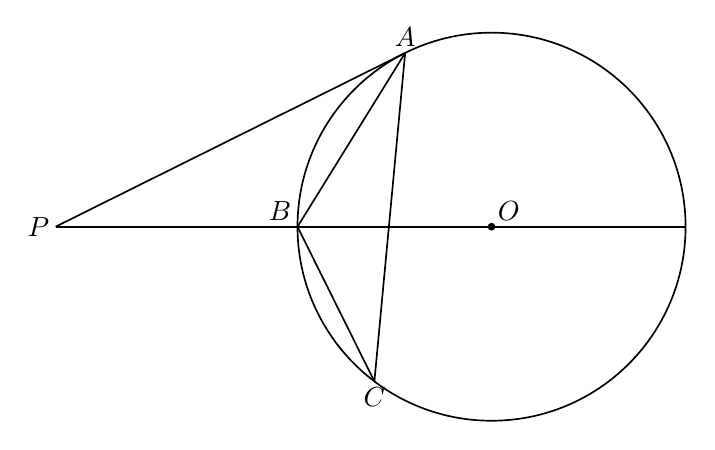
\begin{tikzpicture}[x=1cm,y=1cm,line width=.6pt,font=\normalsize,>=Stealth]
\coordinate (O) at (0.0000000000,0.0000000000);
\coordinate (P) at (-5.5357508034,0.0000000000);
\coordinate (A) at (-1.0969648596,2.2066246168);
\coordinate (B) at (-2.4642491966,0.0000000000);
\coordinate (C) at (-1.4876175273,-1.9645656505);
\coordinate (Q) at (2.4642491966,0.0000000000);
\draw (O) circle[radius=2.4642491966cm];
\draw (P)--(A);
\draw (P)--(Q);
\draw (A)--(B);
\draw (A)--(C);
\draw (B)--(C);
\fill (O) circle[radius=1.4pt];
\node[left=2pt,inner sep=0pt] at (P) {$P$};
\node[above=2pt,inner sep=0pt] at (A) {$A$};
\node[above left=2pt,inner sep=0pt] at (B) {$B$};
\node[below=2pt,inner sep=0pt] at (C) {$C$};
\node[above right=2pt,inner sep=0pt] at (O) {$O$};
\end{tikzpicture}
